\documentclass[12pt]{article}
\usepackage{array,tabularx}
\usepackage{graphicx}
\usepackage{float}
\usepackage{amsmath}
\setlength{\parindent}{0pt}

\newenvironment{conditions}
  {\par\vspace{\abovedisplayskip}\noindent
   \tabularx{\columnwidth}{>{$}l<{$}@{}>{${}}c<{{}$}@{} >{\raggedright\arraybackslash}X}}
  {\endtabularx\par\vspace{\belowdisplayskip}}

\title{Study of Stored Energy and Simple Machines}
\author{Ben Hammond}
\date{\today}


\begin{document}
	\maketitle
	\newpage

	\section{Simple Machines}
	The following six simple machines were invented by humankind in ancient times and are still in use today: the lever, the wheel and axle, the pulley, the inclined plane, the wedge, and the screw. Using your knowledge of forces and energy describe the physics behind each of these simple machines (use free-body diagrams, Newton’s Laws, and equations for work and mechanical energy) and explain why they are so useful. The minimum answer requires one illustration and a paragraph explanation.

	\subsection{The Lever}
	
	\begin{figure}[H]
		\centerline{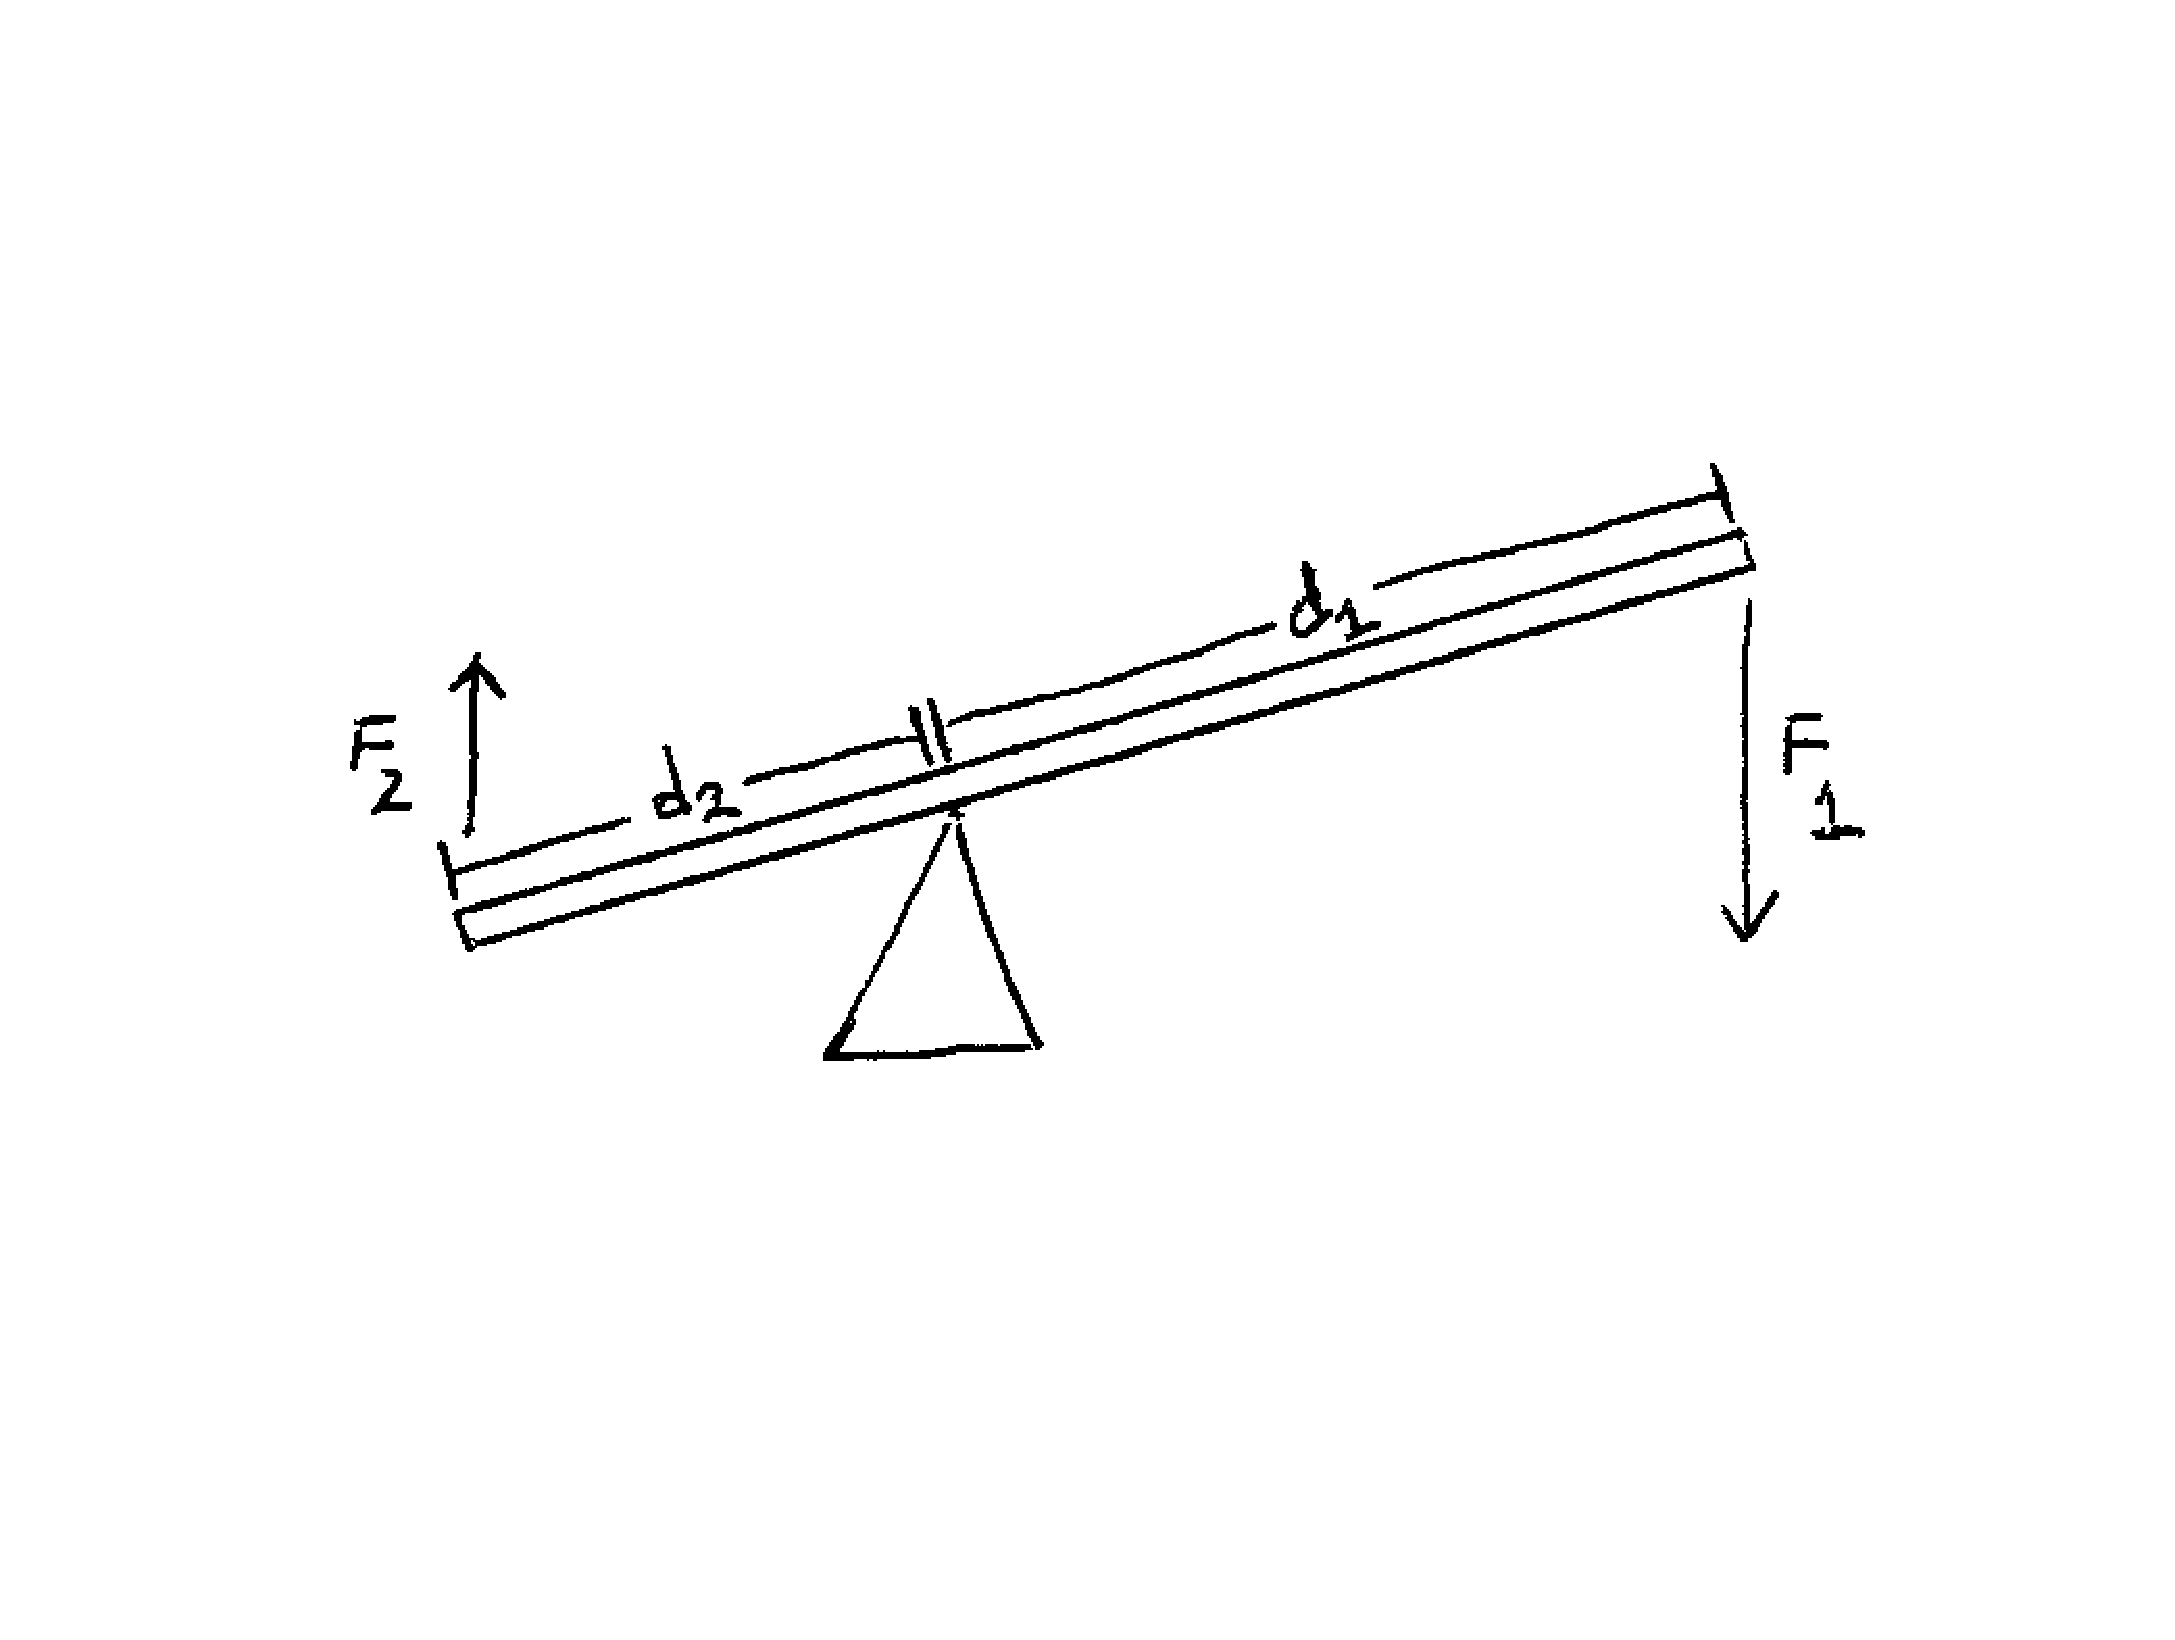
\includegraphics[width=0.5\textwidth]{images/lever.EPS}}
		\caption{A diagram of a lever.}
	\end{figure}

	\paragraph{Description}
	The lever provides a mechanical advantage the same way all simple mechanisms do: by translating distance into force. In the lever, a force $F_1$ exerted downward over distance $d_1$ is translated into a force $F_2$ over distance $d_2$. When distance $d_1$ is larger than distance $d_2$, less force is required to lift an object distance $d_2$, though it is over a longer distance. In this way levers maintain the amount of work done by reducing force and increasing distance.
		
	\subsection{The Wheel and Axle}
	
	\begin{figure}[H]
		\centerline{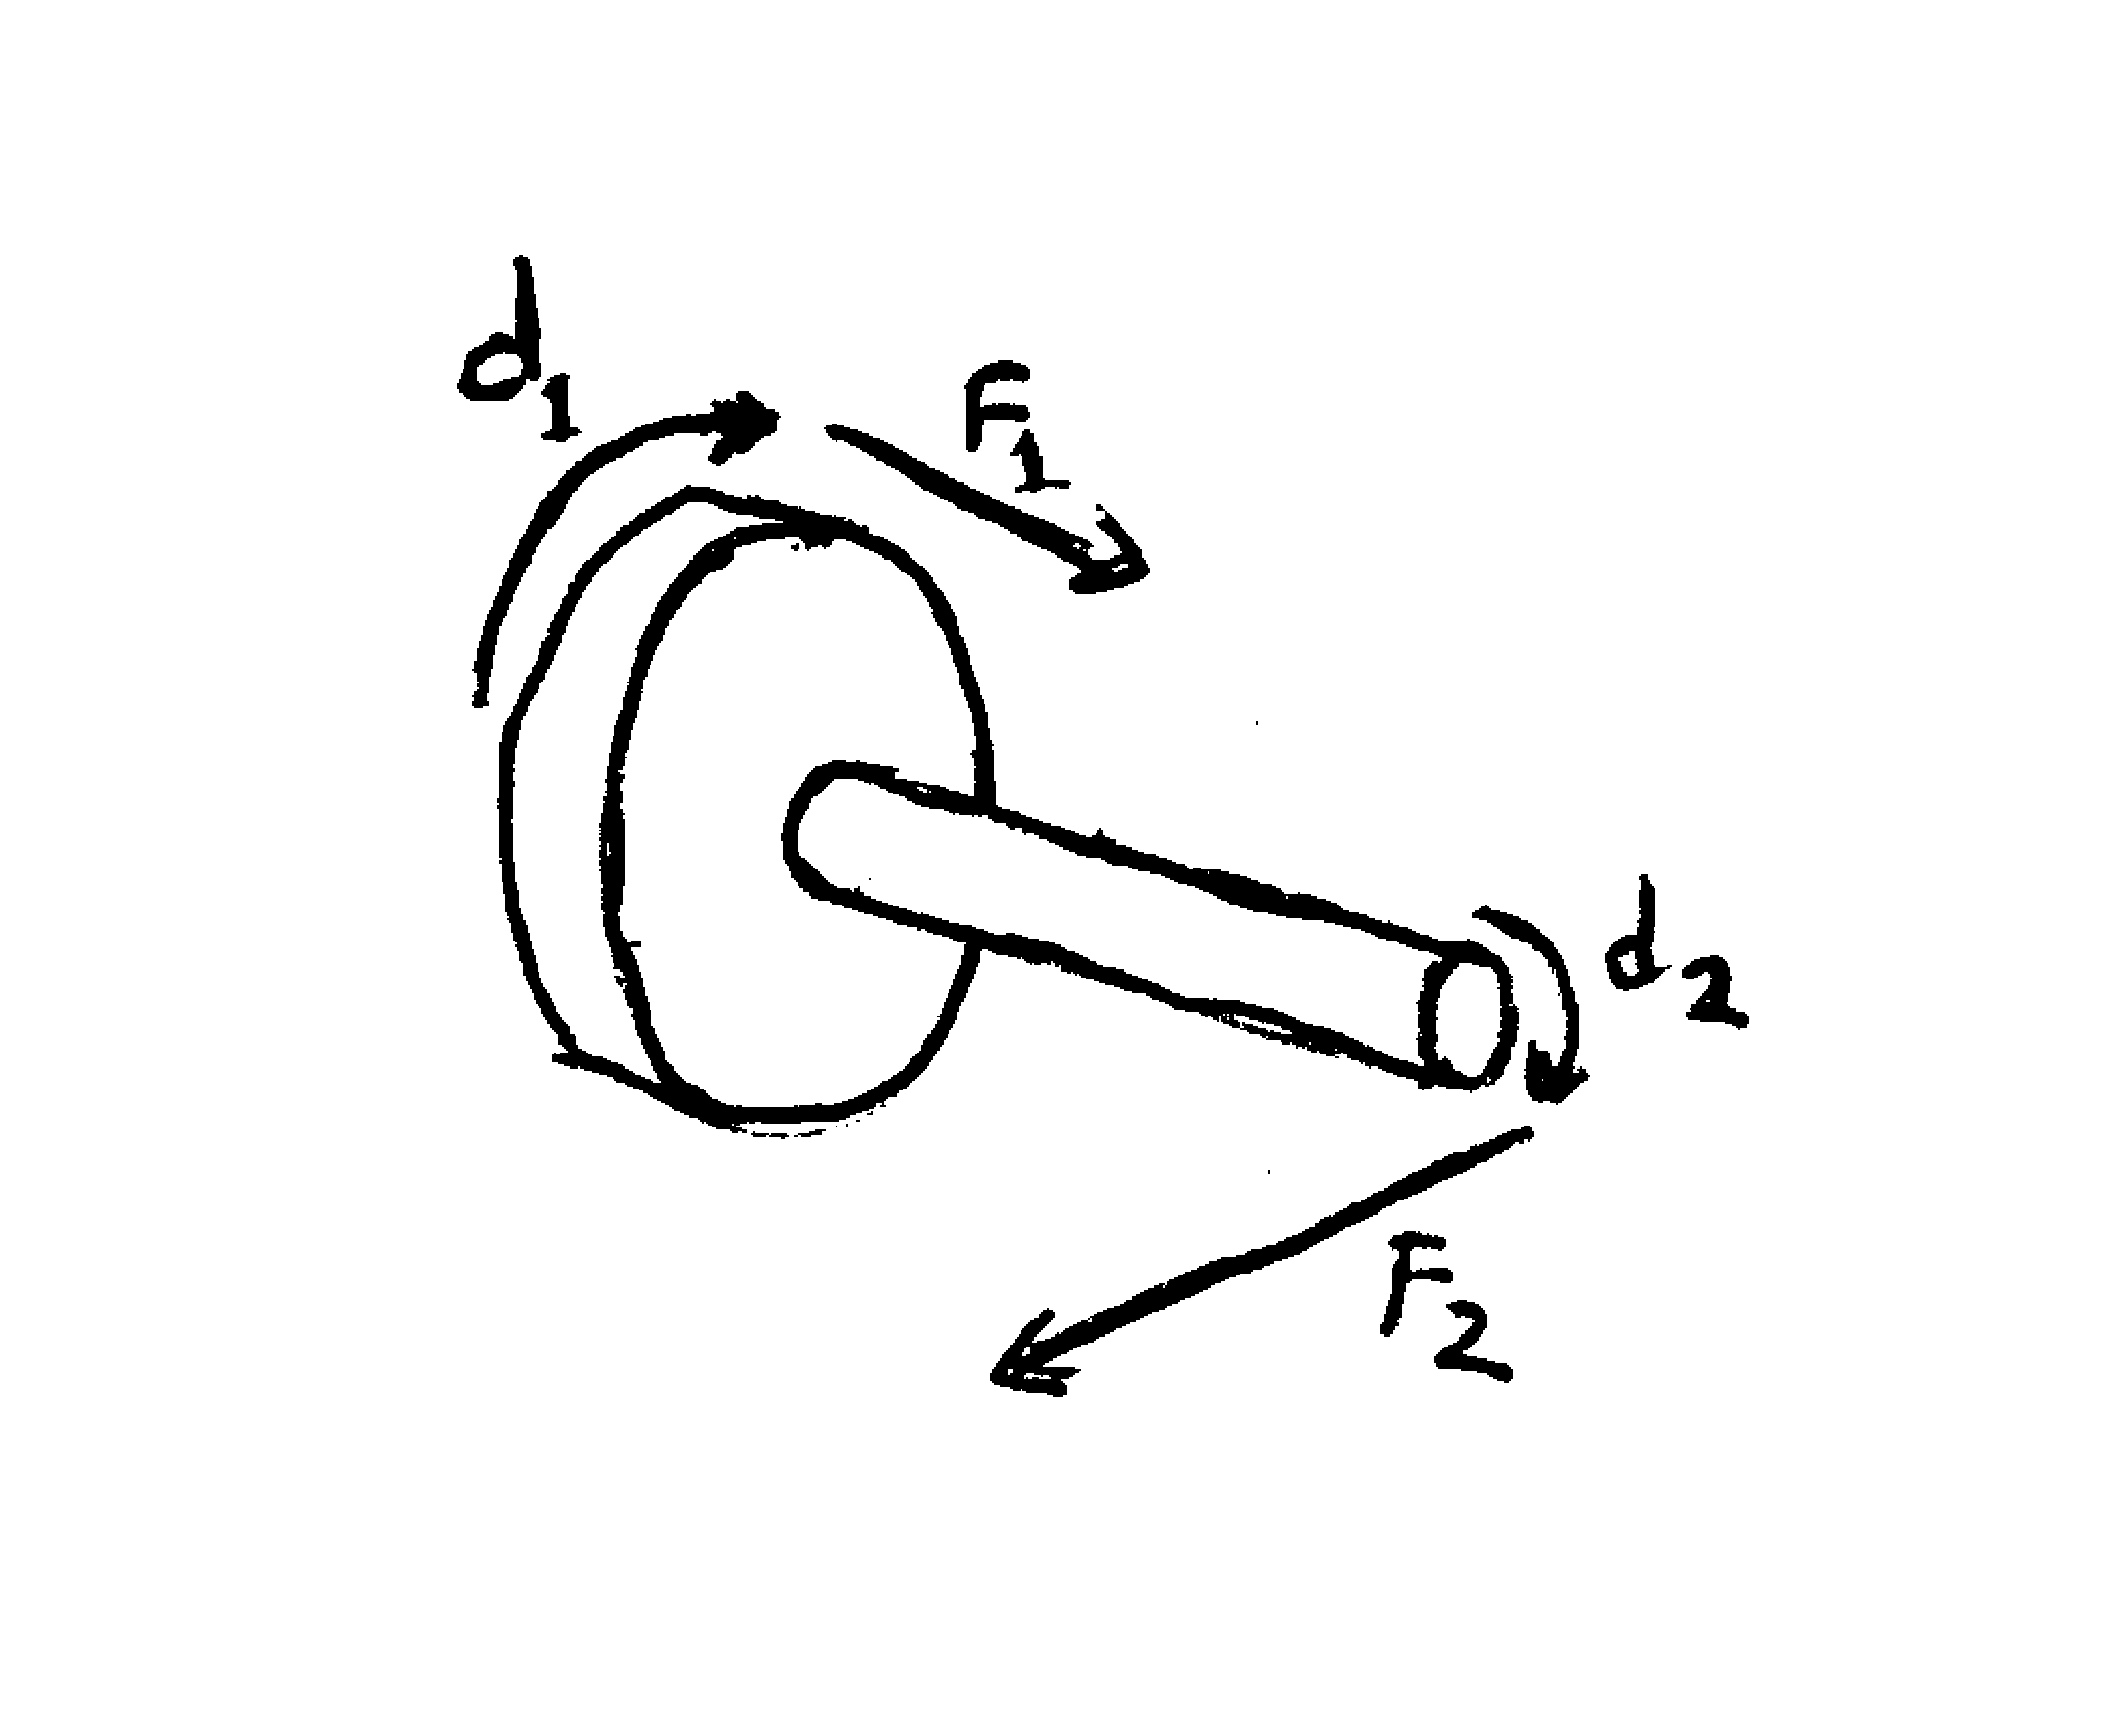
\includegraphics[width=0.5\textwidth]{images/wheel.EPS}}
		\caption{A diagram of a wheel and axle.}
	\end{figure}

	\paragraph{Description}
	The wheel and axle converts distance into force through the use of differently sized cylinders. Because the larger cylinder has to move a larger distance $d_1$ than the smaller cylinder's distance $d_2$, it's force must be smaller. Thus, when a force $F_1$ is applied on the larger cylinder over distance $d_1$, a larger force $F_2$ is applied on the smaller cylinder over a smaller distance $d_2$. In these diagrams the works on each "end" of the mechanism are equal, meaning $F_1 * d_1 = F_2 * d_2$. 
			
	\subsection{The Pulley}
	
	\begin{figure}[H]
		\centerline{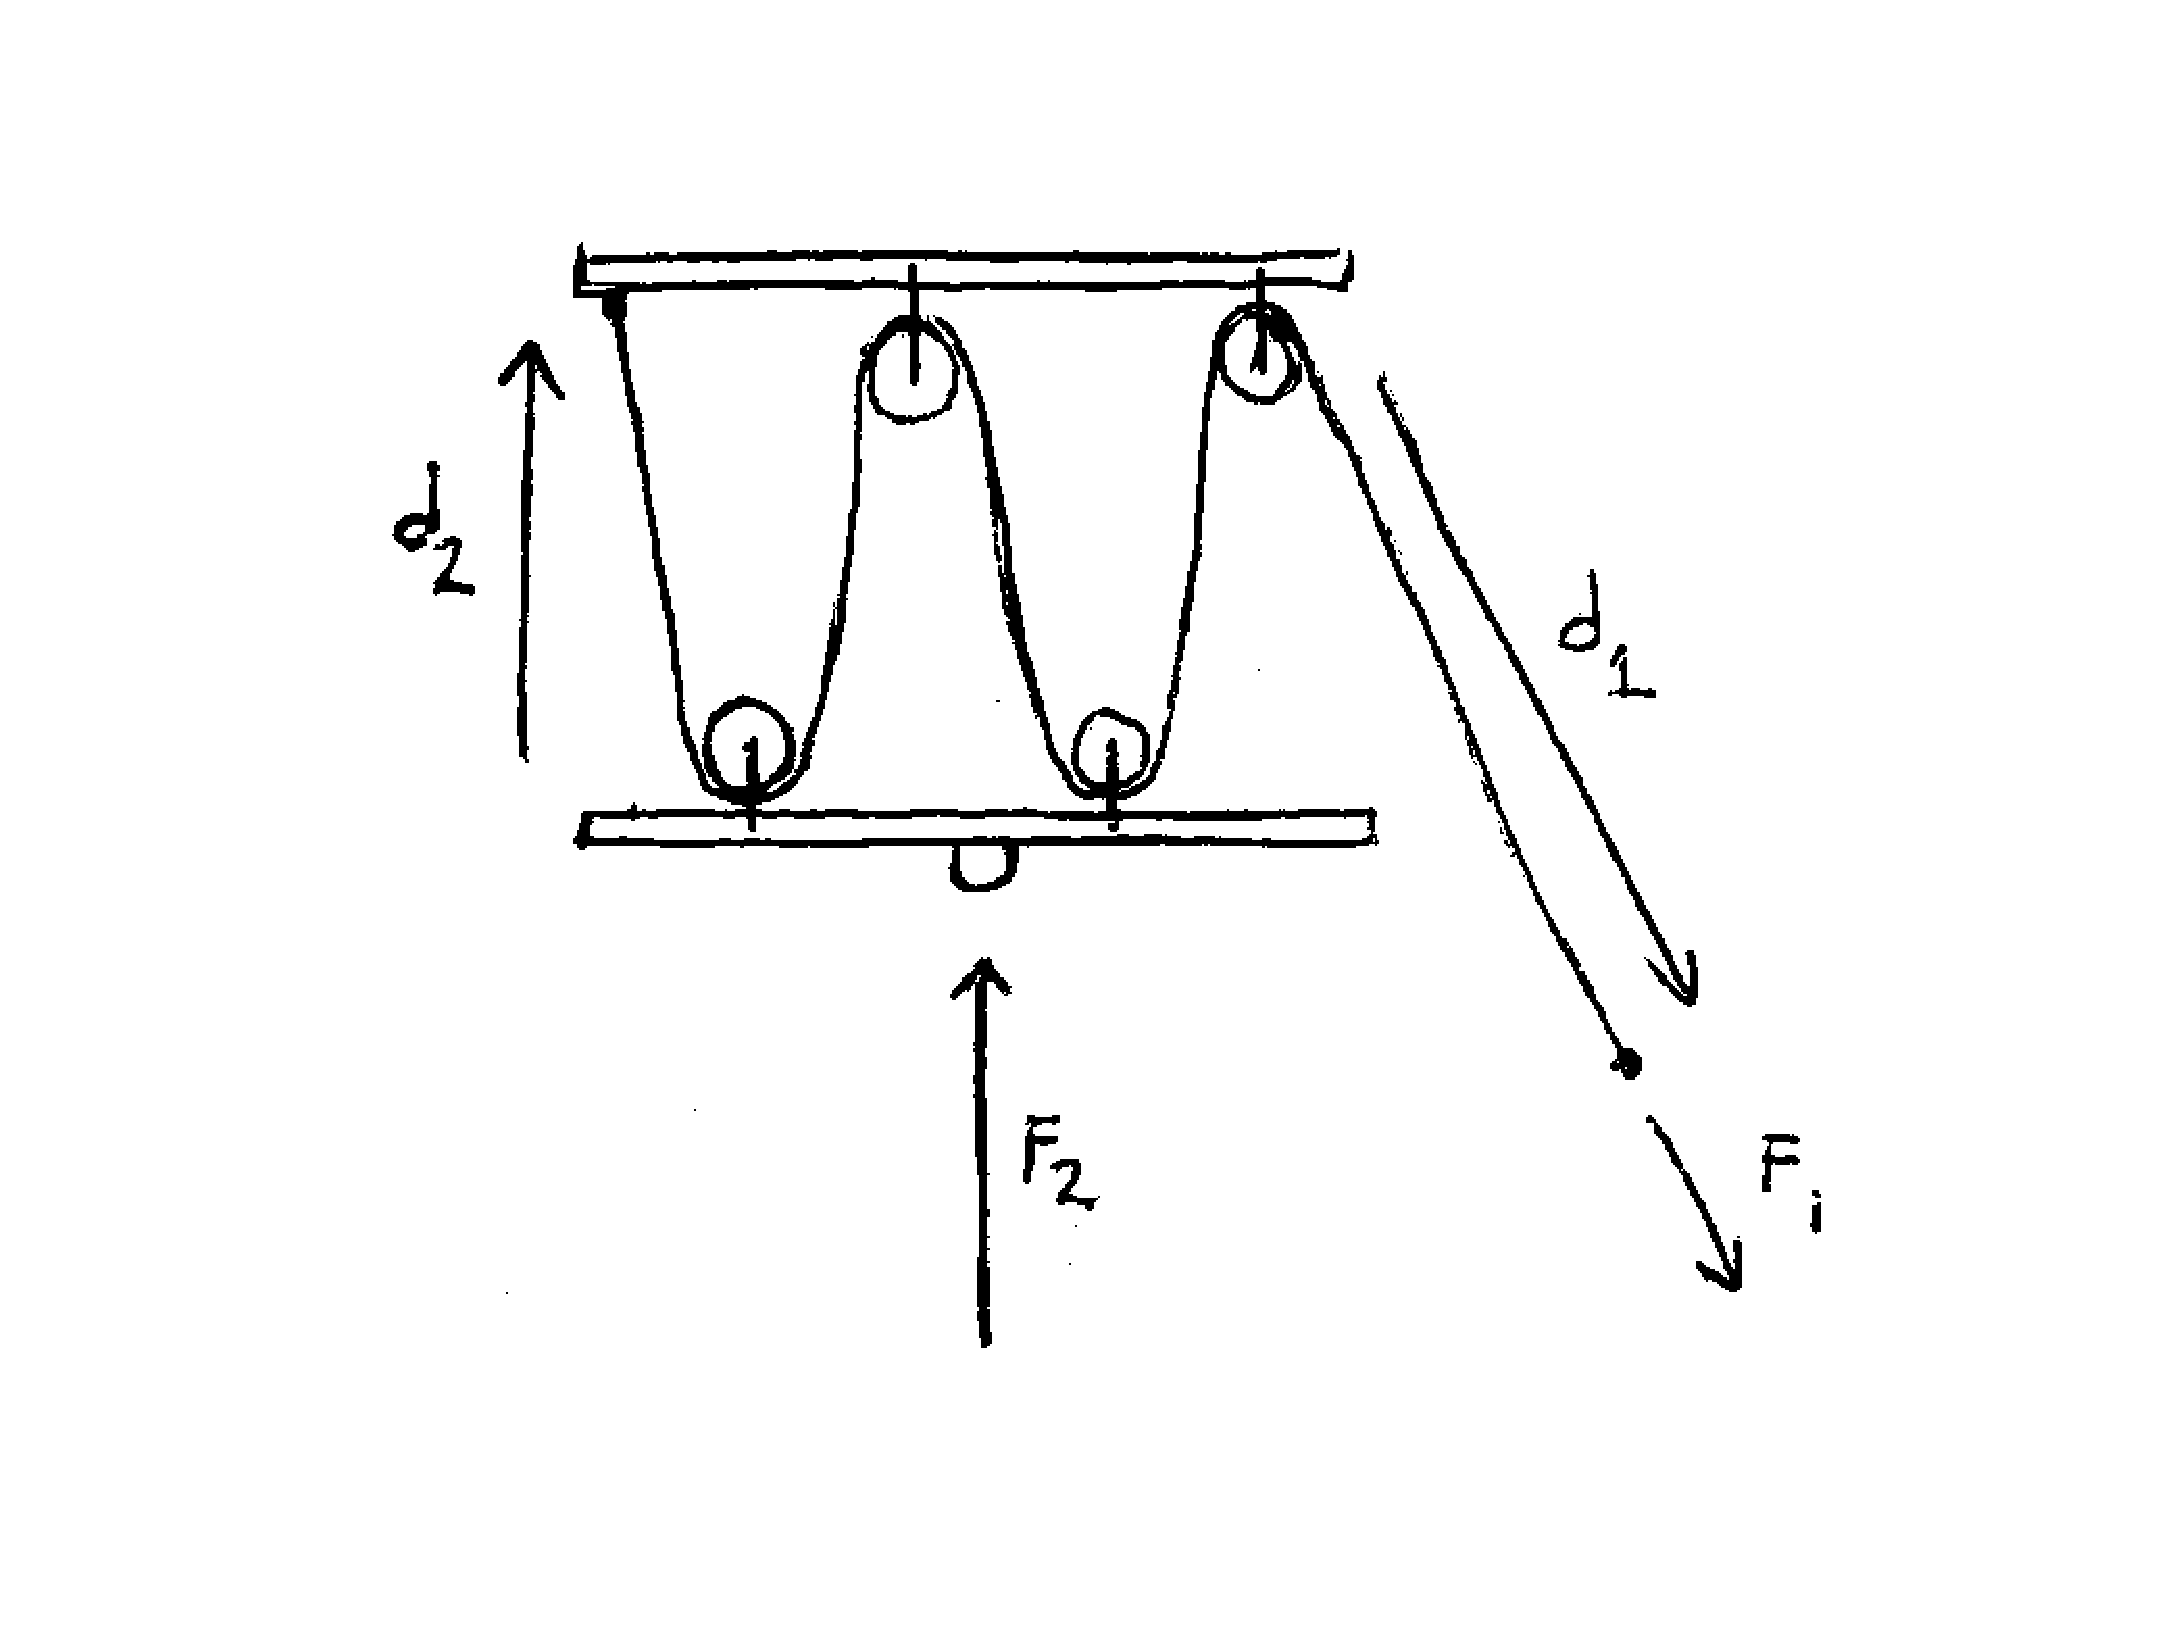
\includegraphics[width=0.5\textwidth]{images/pulley.EPS}}
		\caption{A diagram of a pulley.}
	\end{figure}

	\paragraph{Description}
	The pulley, or block and tackle, is often used to lift heavy objects with little force. As with all other simple mechanisms, this is achieved by increasing the distance over which a smaller force is exerted. The block and tackle does this by increasing the number of pulleys through which the rope passes between the top and the object. This means that to lift the object distance $d_2$, a distance of rope $d_1$ equal to $_2$ multiplied by the number of times the rope loops back and forth, minus one if the end of the rope goes down. For example, in this diagram $d_1$ is equal to $4 * d_2$, because the rope has four lengths connected to the bottom, excluding the one being directly pulled on. As with before, this increase in distance means a corresponding decreasing in force produces the same amount of work.
			
	\subsection{The Inclined Plane}
	\begin{figure}[H]
		\centerline{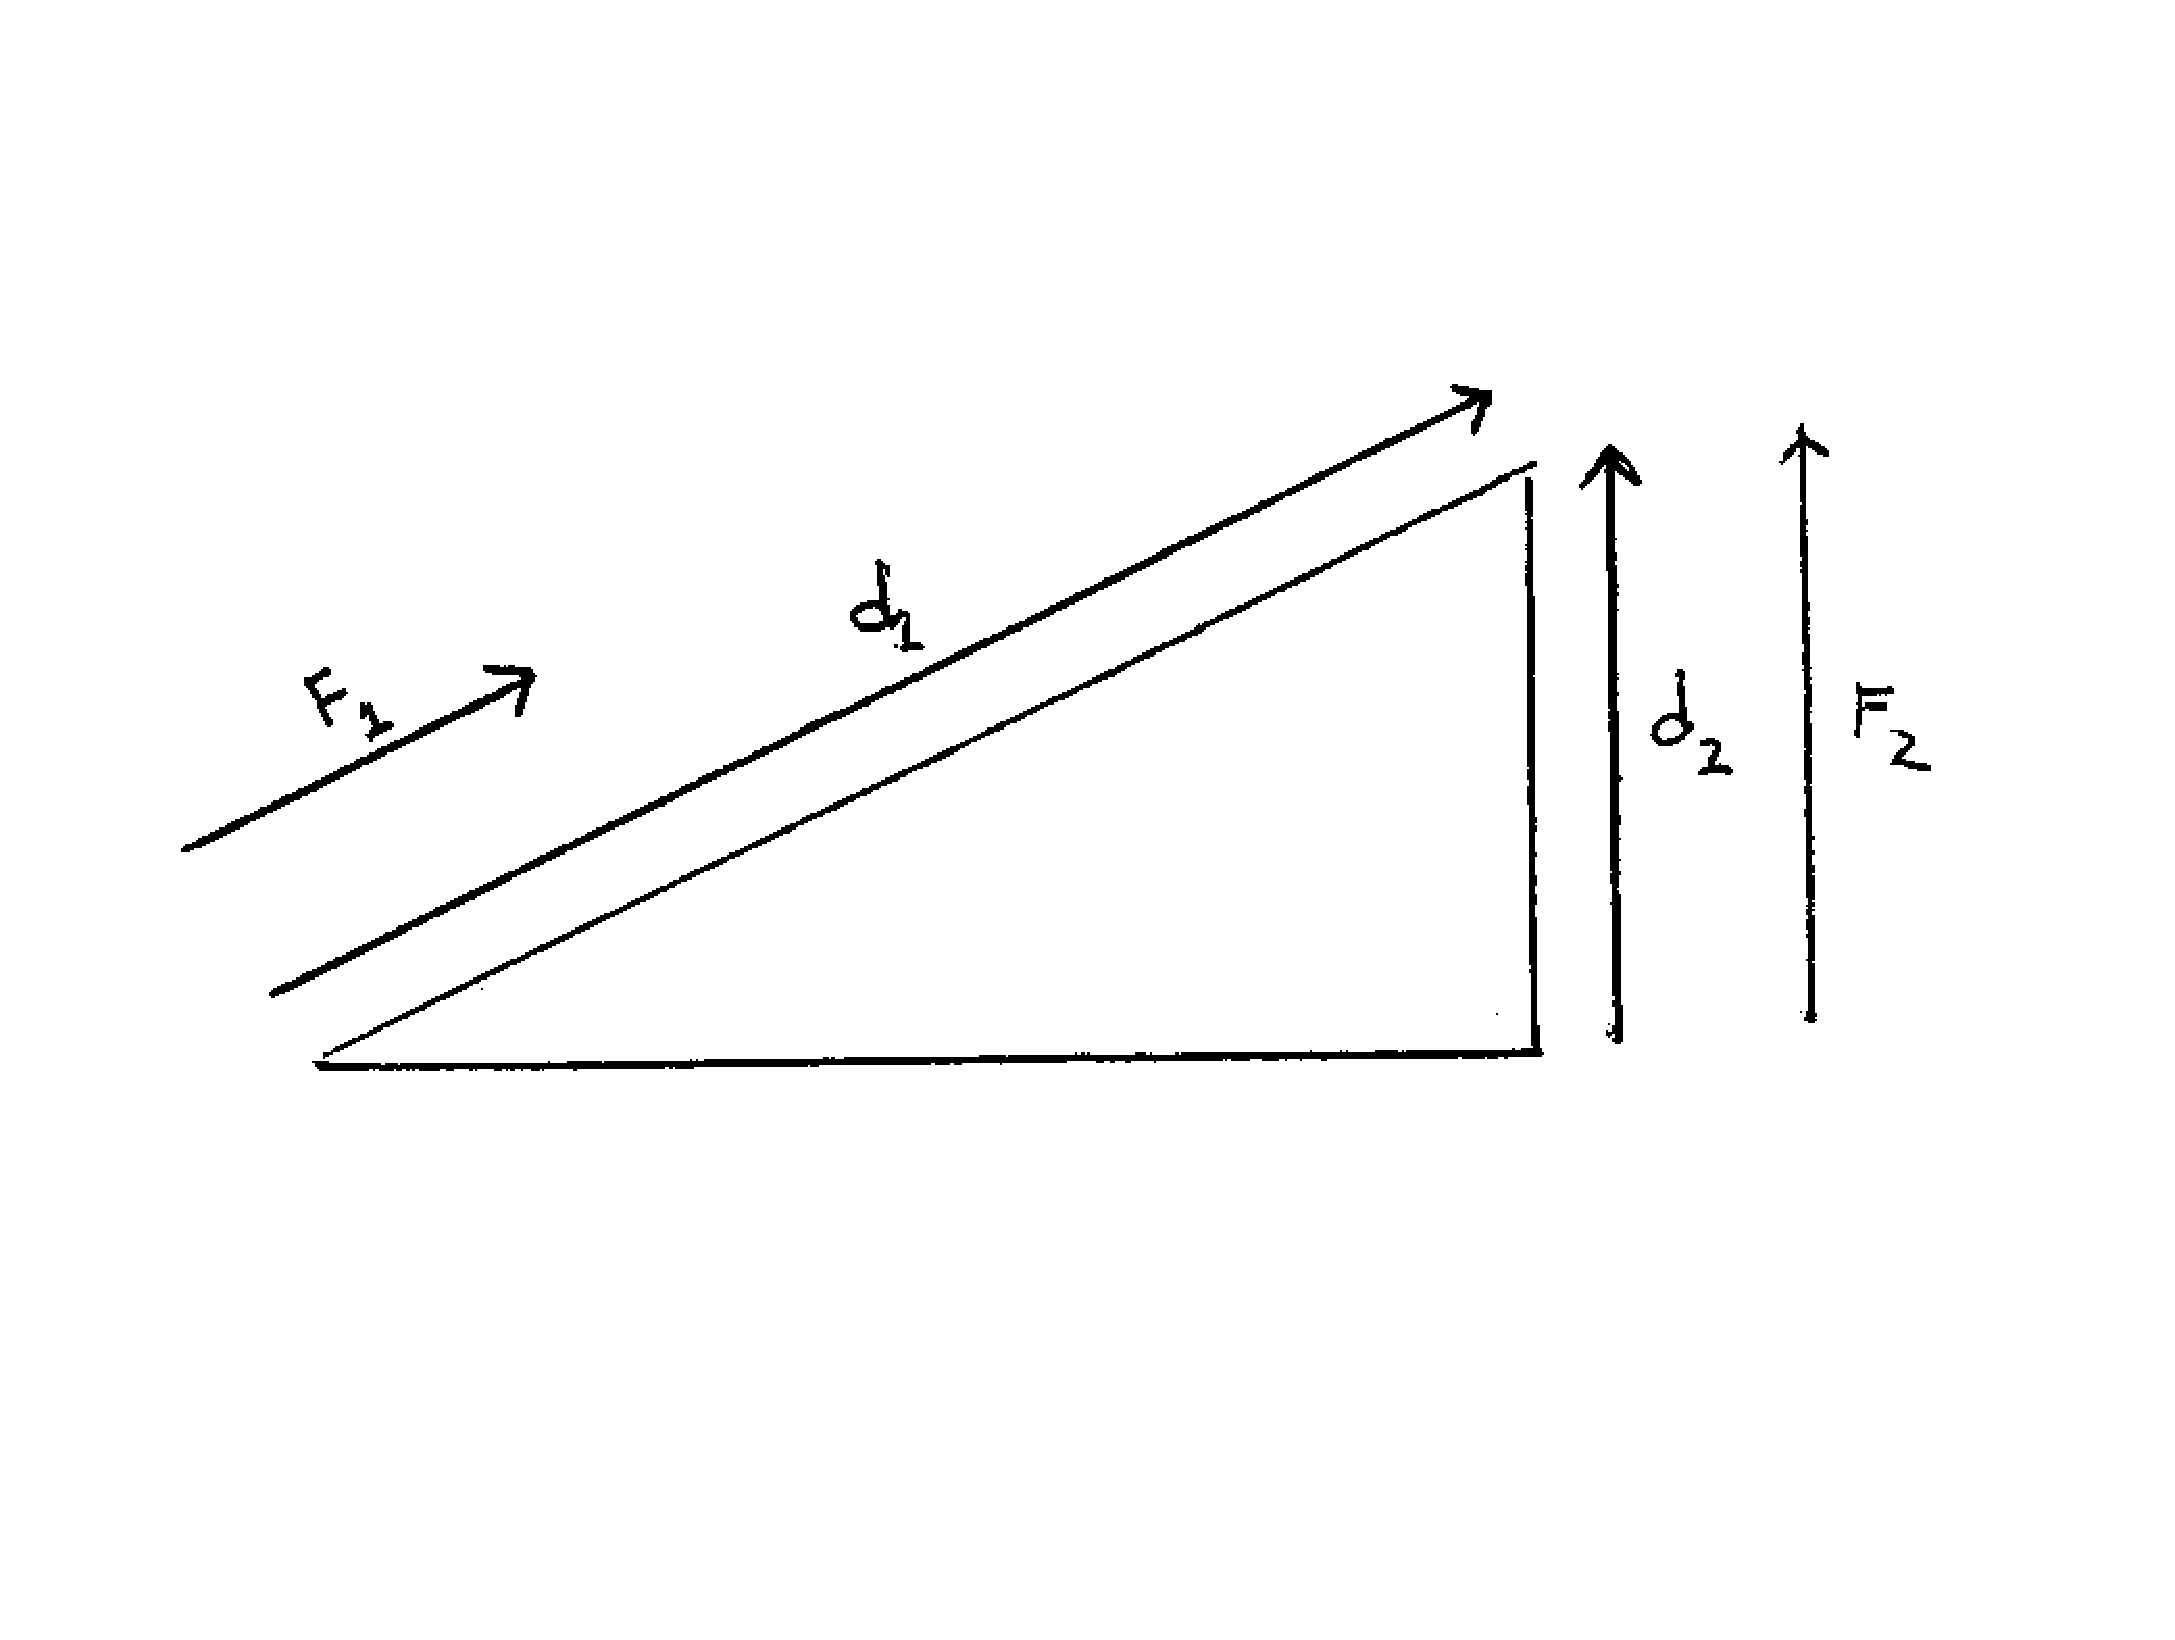
\includegraphics[width=0.5\textwidth]{images/plane.EPS}}
		\caption{A diagram of an inclined plane.}
	\end{figure}
	
	\paragraph{Description}
	Inclined planes are also often used to lift objects, but, unlike with pulleys, they decrease the amount of force necessary to lift an object a height $d_2$ by moving the object in a vertically diagonal line over a longer distance $d_1$. Similarly though, by increasing the distance $d_1$ they decrease the force $F_1$ required to do the same amount of work. This is immensely useful for simply moving heavy objects to a higher elevation, and is how roads going up hills work, extending the distance to decrease the force required of going straight up.
	
	\subsection{The Wedge}
	
	\begin{figure}[H]
		\centerline{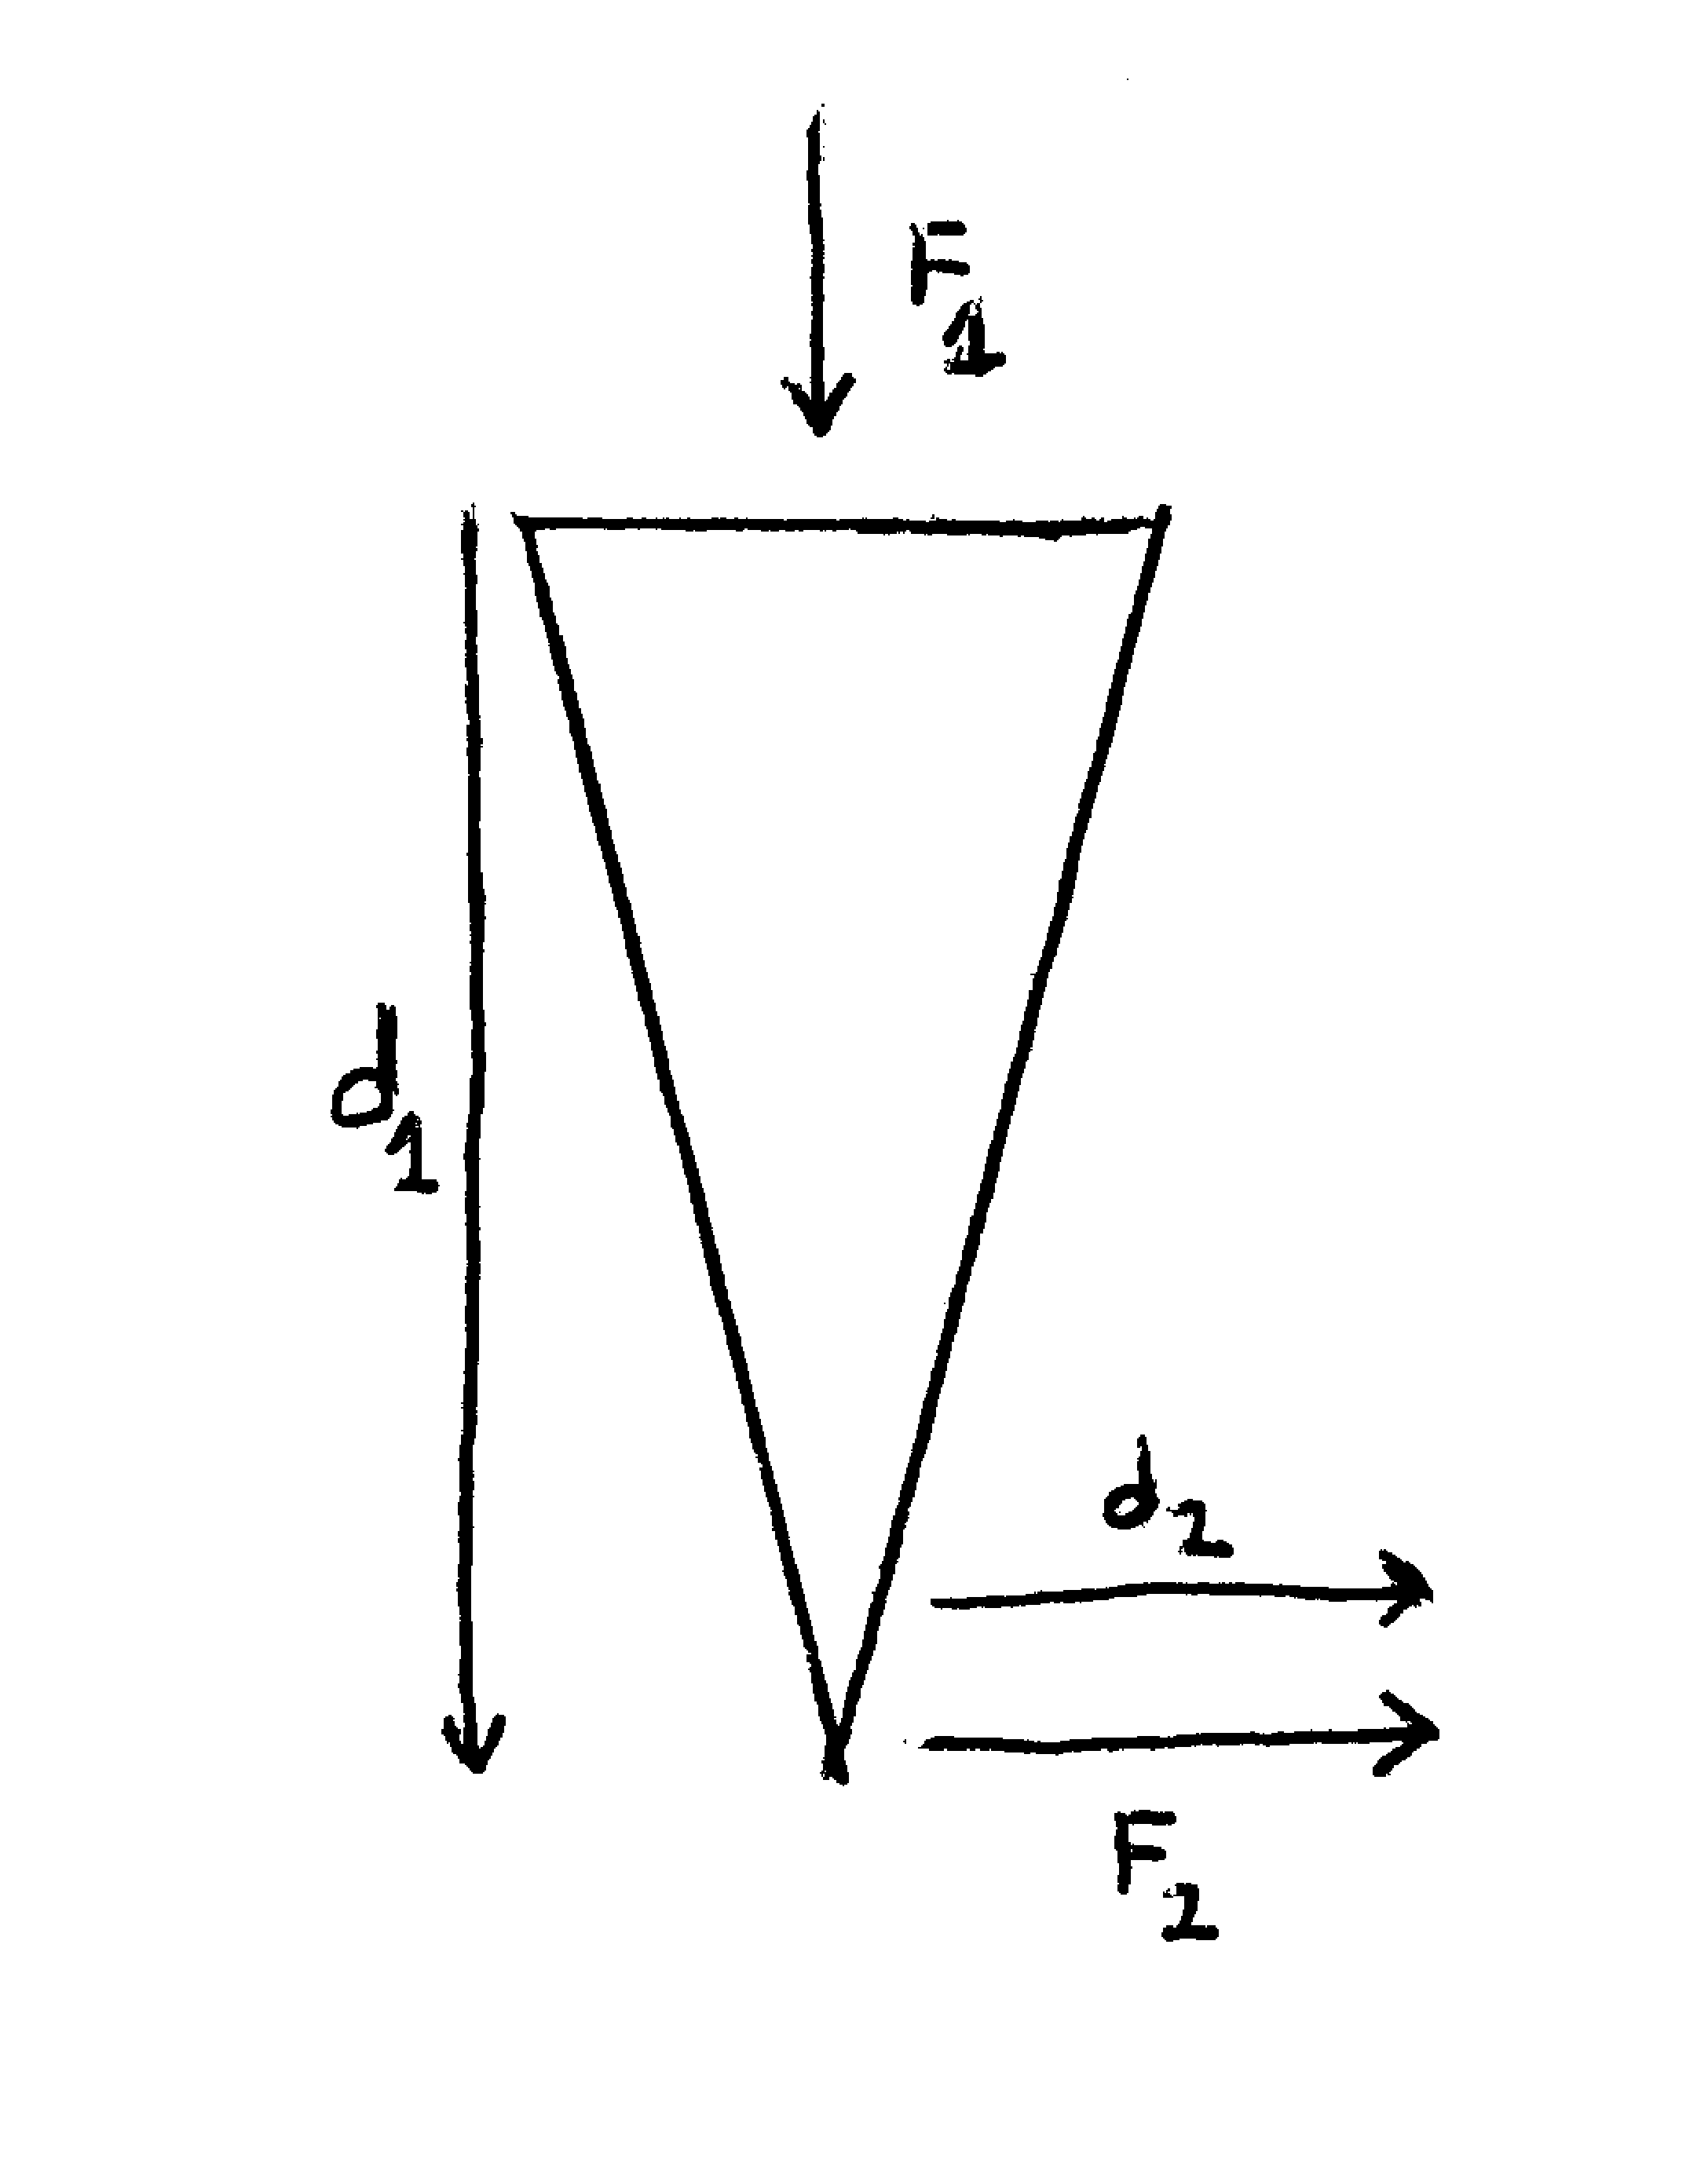
\includegraphics[width=0.5\textwidth]{images/wedge.EPS}}
		\caption{A diagram of a wedge.}
	\end{figure}

	\paragraph{Description}
	An extension of the inclined plane, the wedge uses the same principle of distributing work over larger distances to exert greater forces. This is often used to cut objects, both reducing the amount of force required, and increasing the force exerted. With a wedge, the downward force $F_1$ over distance $d_1$ exerts a larger force $F_2$ over a smaller distance $d_2$ on the surrounding material. Axes, knives, and many other common tools all use the principle of a wedge to make doing work easier and require less force.

	\subsection{The Screw}
	
	\begin{figure}[H]
		\centerline{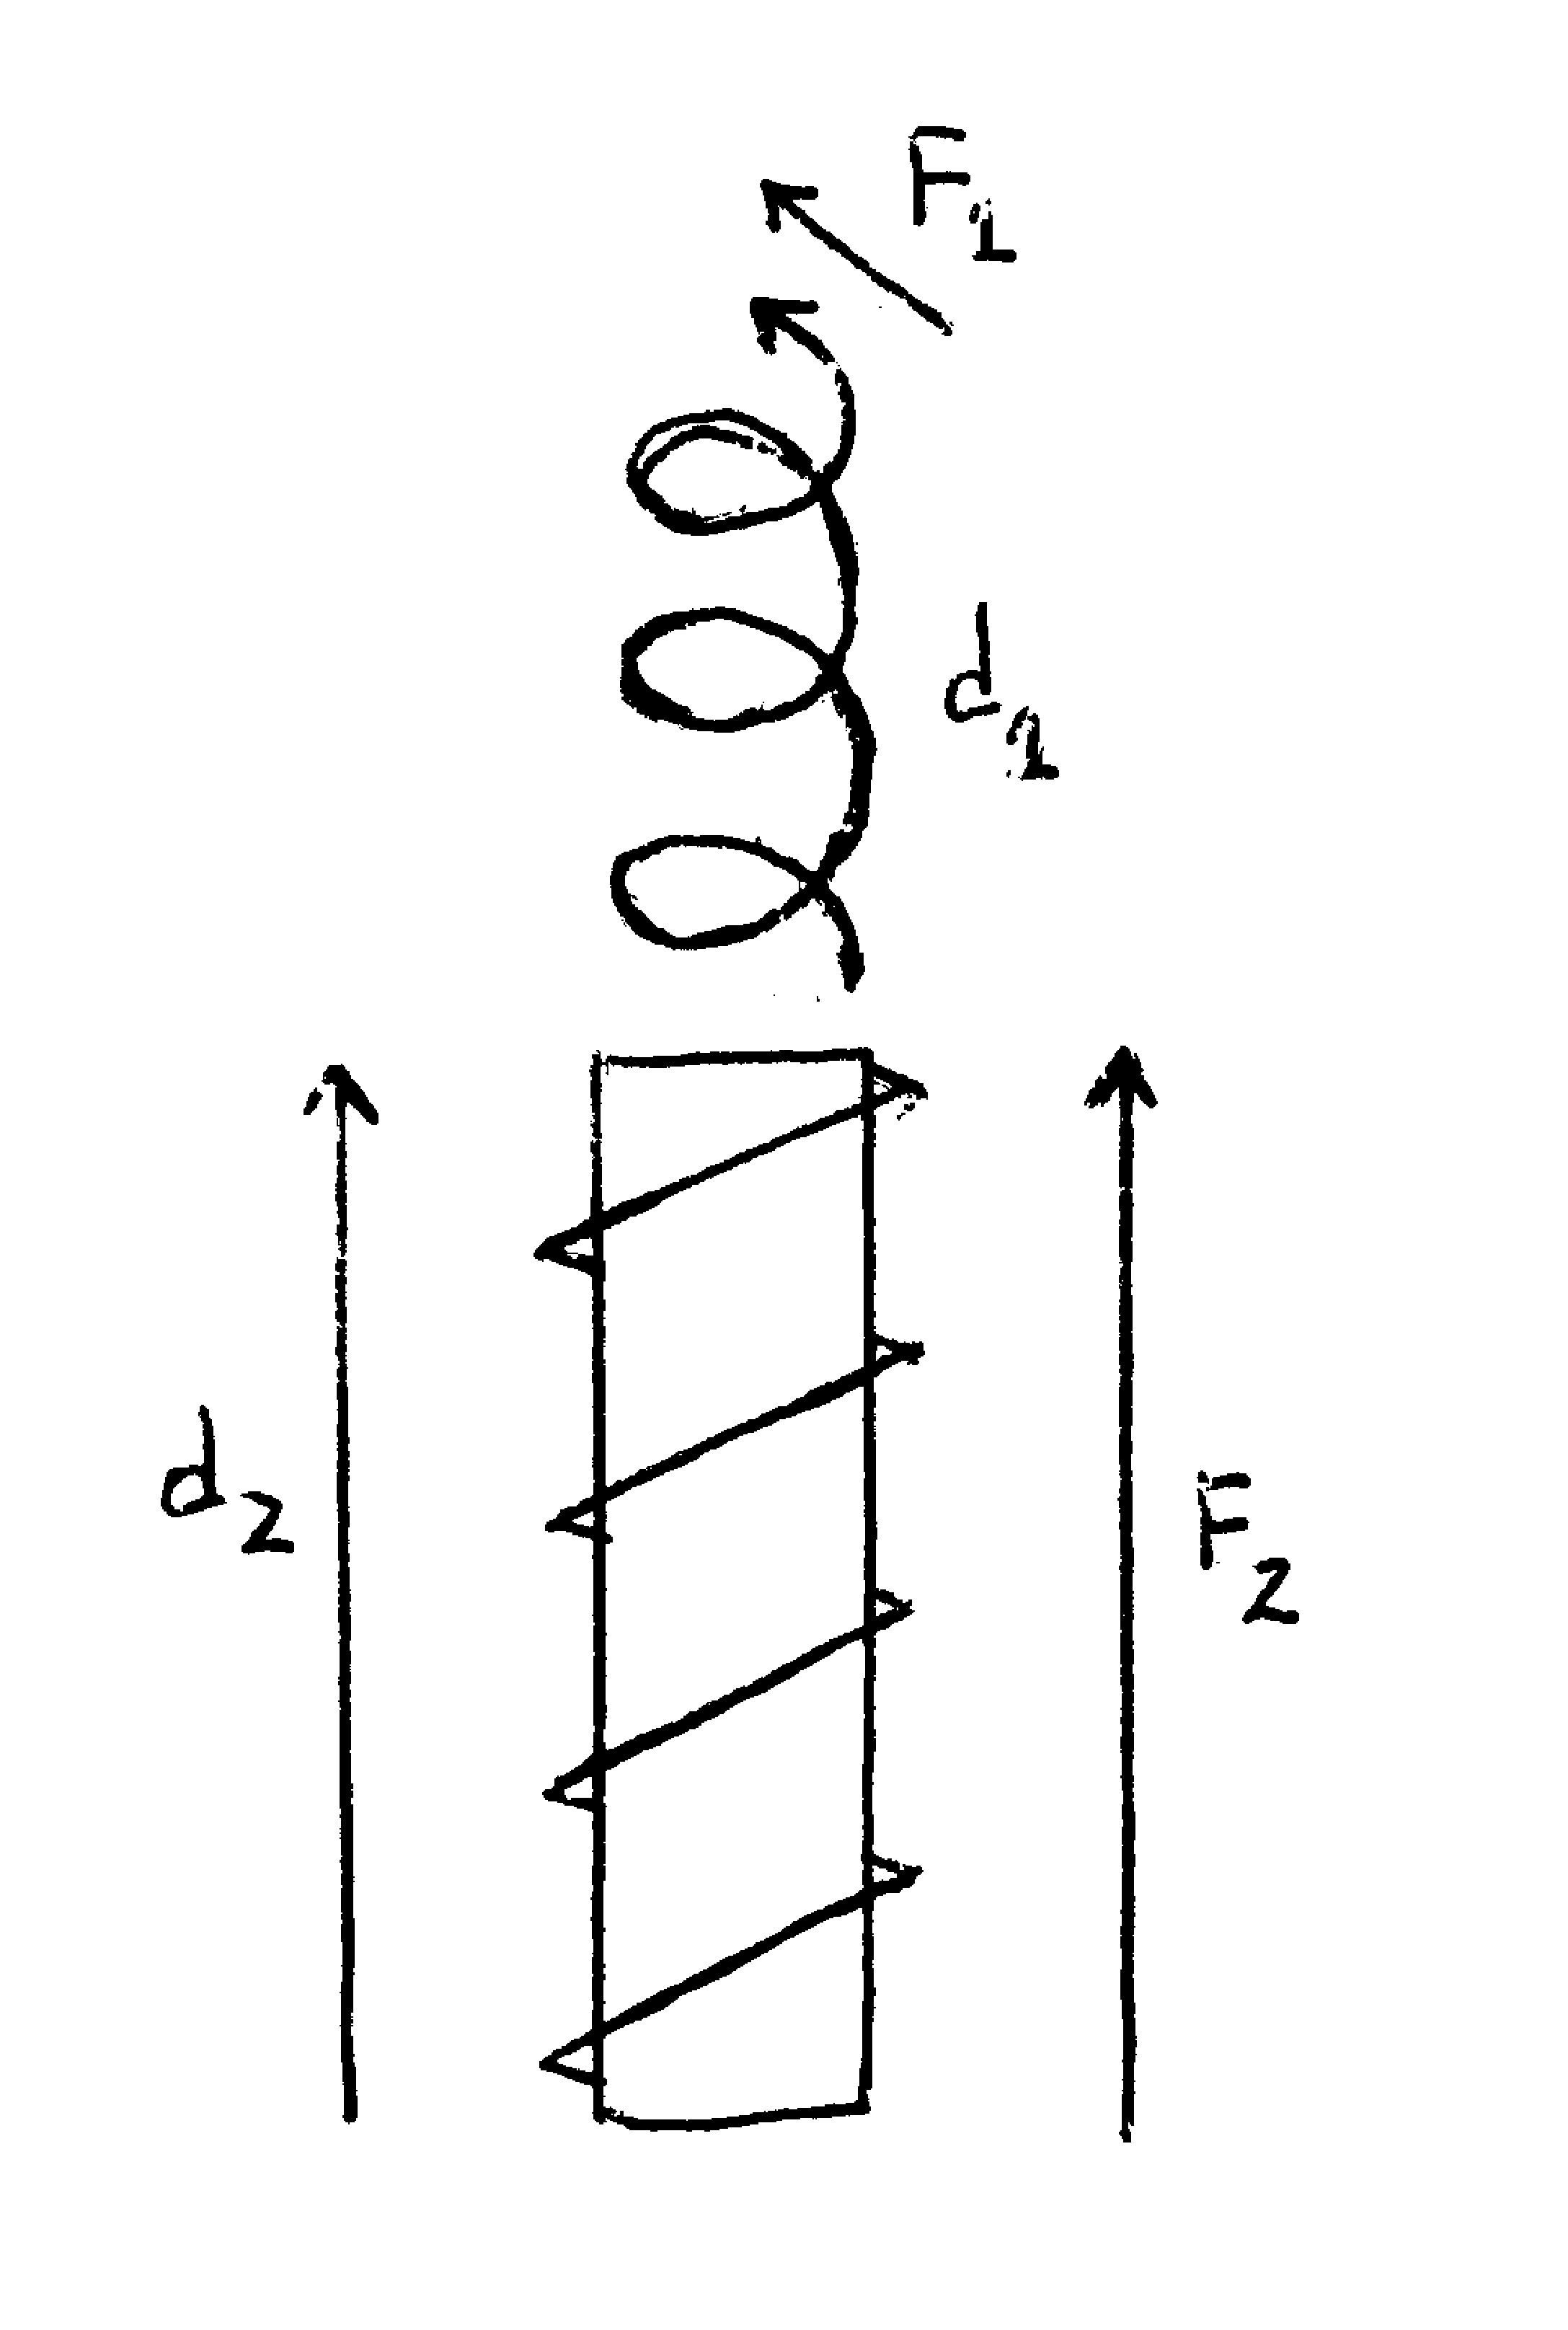
\includegraphics[width=0.5\textwidth]{images/screw.EPS}}
		\caption{A diagram of a screw.}
	\end{figure}
	
	\paragraph{Description}
	Similar to the inclined plane and wedge, the screw translates a rotational force $F_1$ over a rotated distance $d_1$ into a larger vertical force $F_2$ over a shorter vertical distance $d_2$. In some cases this application of force is used to move the screw into a material (in which case the edges of the screw are functioning as wedges), but in others it is used to raise an object, such as with grain elevators or the Archimedes screw.

	
	\section{Energy Storage}
	We have learned that energy can take a number of different forms. In this activity you will design and perform experiments to determine the amount of energy stored in several devices.

	\subsection{Mouse Trap}
	For this device, also estimate the velocity of the end of the bar when the trap is triggered.
	\paragraph{Experimental Design:} The mouse trap was set perpendicular to the ground, and a force gauge was used to measure how much force it took to move the spring loaded bar to parallel with the ground, or at a 90$^{\circ}$ angle to the mouse trap. This force was then used in subsequent calculations to find the spring constant, potential energy, and velocity.
	\paragraph{Data:}
	\begin{flushleft}
	\begin{tabular}{ l|l }
		test & force \\
		\hline
		1 & 0.50 kg \\
		2 & 0.57 kg \\
		3 & 0.59 kg \\
		4 & 0.58 kg \\
		5 & 0.55 kg \\
		avg. & 0.558 kg \\
	\end{tabular}
	\end{flushleft}
	Radius of spring arc: 4.5 cm or 0.045 m
	\paragraph{Calculations:} The first step was to calculate the spring constant from the experimentally found force and distance . This was done first by calculating the arc length of the spring arm to 90$^{\circ}$:
	\begin{equation}
		s = r\theta
	\end{equation}
	$$ s = 0.045 \text{ m} * \frac{1}{2}\pi $$
	$$ s = 0.07069 \text{ m} $$
	With the distance and force now known, the spring constant $k$ was solved for from the Hooke's Law equation
	\begin{equation}
		F = kx
	\end{equation}
	$$ \frac{0.558 \text{ kg}}{9.8 \text{ m/s}^2} = \\
	k * 0.07069 \text{ m} $$
	$$ 0.05694 \text{ N} = k * 0.07069 \text{ m} $$
	$$ k = \frac{0.05694 \text{ N}}{0.07069 \text{ m}} $$
	$$ k = 0.8055 \text{ N/m} $$
	Using this spring constant, the elastic potential energy can be solved for with the equation
	\begin{equation}
		PE = \frac{1}{2}kx^2
	\end{equation}
	and a new arc length
	$$ s = 0.045 \text{ m} * \pi $$
	$$ s = 0.1414 \text{ m} $$
	With known values substituted, the potential energy is solved as follows:
	$$ PE = \frac{1}{2}(0.8055\text{ N/m})(0.1414\text{ m})^2 $$
	$$ PE = 0.4048\text{ N/m} * 0.01999\text{ m}^2 $$
	$$ PE = 0.0081\text{ Nm} = 0.0081\text{ J} $$
	The velocity of the trap when it is triggered can also now be calculated with the equation for kinetic energy 
	
	
	\subsection{Constant Acceleration Cars}
	For this device determine both the energy required to fully "charge" the car and the kinetic energy of the car when it is released. The percent efficiency of the device is the energy released divided by the energy required to charge it multiplied by 100.
	\paragraph{Experimental Design:} The car was fully wound up, and placed on an inclined surface. The surface's angle was then slowly lowered until the car accelerated, and then that angle was measured. The mass of the car was also measured. Separately, the distance it took to wind the car was measured. The time it took to unwind that distance was also recorded.
	\paragraph{Data:}
	\begin{flushleft}
	\begin{tabular}{ l|l }
		angle & 5$^{\circ}$ \\
		\hline
		mass of car & 0.11437 kg \\
		\hline
		winding dist. & 0.40 m \\
		\hline
		time to unwind & 7 s \\
	\end{tabular}
	\end{flushleft}
	\paragraph{Calculations:} By finding the force of gravity acting on the car at a 5$^{\circ}$ angle, the force of the spring can also be found:
	\begin{equation}
		F = mg \sin(\theta)
	\end{equation}
	$$ F = 0.11437 \text{ kg} * 9.8 \text{ m/s}^2 * \sin(5) $$
	$$ F = 0.09769 \text{ N} $$
	Then, by multiplying the force by the winding distance, the potential energy was found
	$$ PE = 0.09769 \text{ N} * 0.40 \text{ m} $$
	$$ PE = 0.03908 \text{ J} $$
	The average velocity of the car was found through the equation
	\begin{equation}
		\bar{v} = \frac{\Delta t}{\Delta x}
	\end{equation}
	$$ \bar{v} = \frac{0.40 \text{ m}}{7 \text{ s}} $$
	$$ \bar{v} = 0.5714 \text{ m/s} $$
	the result of which was then multiplied by two to find the final velocity:
	$$ v_f = 2 * 0.5714 \text{ m/s} $$
	$$ v_f = 0.1143 \text{ m/s} $$
	With that velocity, the kinetic energy was found
	\begin{equation}
		KE = \frac{1}{2}mv^2
	\end{equation}
	$$ KE = \frac{1}{2} 0.11437 \text{ kg} (0.1143 \text{ m/s})^2 $$
	$$ KE = 0.05719 \text{ kg} 0.01306 \text{ (m/s)}^2 $$
	$$ KE = 7.471 \times 10^-4 \text{ J} $$
	The efficiency was then found through
	\begin{equation}
		\text{efficiency} = \frac{KE}{PE}*100\%
	\end{equation}
	$$ \text{efficiency} = \frac{7.471 \times 10^-4 \text{ J}}{0.3908 \text{ J}}*100\% $$
	$$ \text{efficiency} = 1.912\% $$
	
	\subsection{Household Item (Rubber Band)}
	Experimentally determine the energy stored in the device and the device's efficiency.
	\paragraph{Experimental Design:}
	\paragraph{Data:}
	\paragraph{Calculations:}
	
	\subsection{Nerf Gun}
	Experimentally determine the work required to fully charge the Nerf Gun, the kinetic energy of the projectile, and the Nerf Gun's efficiency.
	\paragraph{Experimental Design:} The force required to pull back the action was measured, as well as the distance it was pulled. The Nerf Gun was then placed at 0$^{\circ}$ and 0.36 m above the ground, and was fired, ten times to find an average.
	\paragraph{Data:}
	\begin{flushleft}
	\begin{tabular}{ l|l }
		force & 10. N \\
		\hline
		distance & 0.017 m \\
		\hline
		action dist. & 0.054 m
	\end{tabular} \\
	\begin{tabular}{ l|l }
		test & distance \\
		\hline
		1 & 1.65 m \\
		2 & 1.73 m \\
		3 & 1.79 m \\
		4 & 1.81 m \\
		5 & 1.87 m \\
		6 & 1.96 m \\
		7 & 1.98 m \\
		8 & 2.00 m \\
		9 & 2.06 m \\
		10 & 2.15 m \\
		avg. & 1.900 m \\
	\end{tabular}
	\end{flushleft}
	\paragraph{Calculations:}
	With the distance and force known, the spring constant $k$ was solved for from the Hooke's Law equation
		\begin{equation}
			F = kx
		\end{equation}
		$$ 10. N = k * 0.017 \text{ m} $$
		$$ k = \frac{10. \text{ N}}{0.017 \text{ m}} $$
		$$ k = 588.2 \text{ N/m} $$
		Using this spring constant, the elastic potential energy can be solved for with the equation
		\begin{equation}
			PE = \frac{1}{2}kx^2
		\end{equation}
		and the total distance of the action
		$$ PE = \frac{1}{2}(588.2\text{ N/m})(0.054\text{ m})^2 $$
		$$ PE = 294.1\text{ N/m} * 0.002916\text{ m}^2 $$
		$$ PE = 0.8576\text{ Nm} = 0.8576\text{ J} $$
		The time the dart took to drop was solved with the 2d motion equation
		\begin{equation}
			t = \sqrt{2 * \frac{x}{9.8\text{ m/s}^2}}
		\end{equation}
		$$ t = \sqrt{2 * \frac{0.36\text{ m}}{9.8\text{ m/s}^2}} $$
		$$ t =  0.27\text{ s} $$
	
\end{document}
